\begin{frame}{Bhatnagar-Gross-Krook Theory}
  \vspace{0.5cm}
  \begin{columns}
   \column{0.5\textwidth}
    \vspace{0.5cm}
     \begin{itemize}
      \item The collisional operator of the Boltzmann equation takes the form\cite{bhatnagar1954model}$\hspace{-0.3cm}^,$\cite{sun2014validity}
      \begin{align*}
        \left[  \pdiff{ f }{t} \,\right]_\text{BGK} =
        \nu \left( f_M - f \,\right).
      \end{align*}
      \item $\nu$ is the relaxation rate.
      \item $f$ is the current distribution.
      \item $f_M$ is the Maxwell-Boltzmann distribution.
      \item Assuming an infinite medium and no external forces.
    \end{itemize}
    \column{0.5\textwidth}
    \vspace{0.5cm}
      \begin{align*}
        \pdiff{ f }{t} =
        \nu \left( f_M - f \,\right)
      \end{align*}
      \vspace{-0.75cm}
        \begin{align*}
          f\,(t) = f_M +
          e^{-\nu t} \left( f\,(0) - f_M \right)
        \end{align*}
        \begin{itemize}
        \item Maxwell molecules are used.
          \begin{align*}
            \sigma =
            \frac{ \sigma_0 }{ c_r }
          \end{align*}
        \item $\sigma_0$ is the reference cross section.
        \item $c_r$ is the relative speed between colliding particles.
      \end{itemize}
  \end{columns}
\end{frame}


\begin{frame}{Relaxation Rate from Collision Frequency}
  \begin{columns}
    \column{0.5\textwidth}
    \begin{itemize}
      \item The relaxation rate $\nu$ can be related to the collision frequency $\nu_0$ \cite{gallis2011investigation}
        \begin{align*}
          \frac{ \nu }{ \nu_0 }
          =
          \frac{
            \alpha \left( 5 - 2 \omega \right) \left( 7 - 2 \omega \right) \text{Pr}
          }{
            5 \left( \alpha + 1 \right) \left( \alpha + 2 \right) \frac{ \mu_\infty }{ \mu_1 }
          }.
        \end{align*}
      \item Temperature viscosity exponent $\omega = 1$.
      \item Angular scattering component $\alpha = 2.13986$.
    \end{itemize}
    \column{0.5\textwidth}
    \begin{itemize}
      \item Infinite to first approximation from Chapman-Enskog theory $\mu_\infty / \mu_1 = 1$.
      \item Prandtl number Pr$ = 1$.
      \item This yields an analytic relaxation rate $\nu$:
      \begin{align*}
        \nu = 0.49387 \nu_0.
      \end{align*}
    \end{itemize}
  \end{columns}
\end{frame}

\begin{frame}{BGK Problem Setup}
  \vspace{1cm}
  \begin{columns}
    \column{0.5\textwidth}
    \begin{itemize}
        \item Simulated on a $100\times100$ grid where $x, y \in [0, 1] \times 10^{6}$ $\text{\fontfamily{STIX2Text-TLF}\selectfont m}$ with reflective boundary conditions.
        \item Neutral argon particles are utilized.
        \item Number density: $n = 1$ $\text{\fontfamily{STIX2Text-TLF}\selectfont m}^{-3}$.
        \item Time step: $\Delta t = 0.01$ $\text{\fontfamily{STIX2Text-TLF}\selectfont s}$.
        \item Particles per element: $N_p = 400$.
%    \begin{align*}
%      f_0 =
%      \prod_{i = 0}^2
%      \sqrt{\frac{ m }{ 2 k_B T_i }}
%      \exp \left( - \frac{ m v_i^2 }{ 2 k_B T_i } \right)
%    \end{align*}
      \item One component starts at $373$ $\text{\fontfamily{STIX2Text-TLF}\selectfont K}$ and the others are at $273$ $\text{\fontfamily{STIX2Text-TLF}\selectfont K}$.
      \item All components thermalize over time.
    \end{itemize}
    \column{0.5\textwidth}
    \begin{figure}[H]
      \centering
      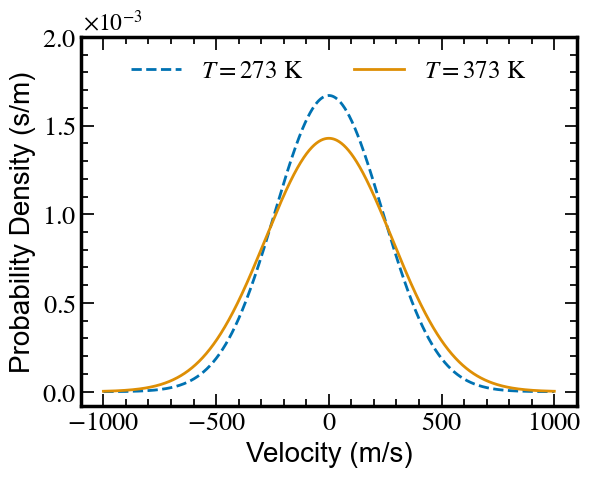
\includegraphics[width=\textwidth]{figs/bgk_ic.png}
    \end{figure}
  \end{columns}
\end{frame}

\begin{frame}{BGK Relaxation Results}
  \begin{columns}
    \column{0.5\textwidth}
    \begin{itemize}
        \visible<1->{
        \item Repeated $10$ times with a different seed value for the pseudorandom number generators.
        \item Each set of $10$ simulations is also repeated, cycling the high temperature through components.
        }
        \visible<3->{
        \item Simulated relaxation rate: $0.49094 \pm 0.02733$.
        \item Error from theory $0.59372\%$.
        }
    \end{itemize}
    \column{0.5\textwidth}
    \visible<2->{
    \vspace{1cm}
    \begin{figure}[H]
      \centering
      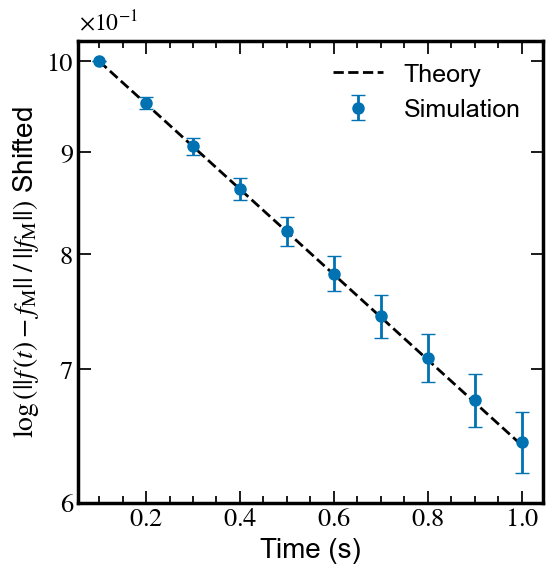
\includegraphics[width=0.9\textwidth]{figs/bgk.png}
    \end{figure}
    }
  \end{columns}
\end{frame}
